\documentclass[]{report}   % list options between brackets
\usepackage[margin=1in]{geometry}
\usepackage{color}
\usepackage{setspace}
\usepackage{datatool, filecontents}
\usepackage{amsmath}
\usepackage{amsfonts}
\usepackage{tabularx}
\usepackage{array,multirow,graphicx}
\usepackage{makecell}
\usepackage{caption,setspace}
\usepackage{float}


% type user-defined commands here



\begin{document}
\setstretch{1.3}{}
%\title{NEON NIST Data Science Evaluation Report}   % type title between braces
%\author{University of Florida}         % type author(s) between braces
%\date{October 27, 2017}    % type date between braces
%\maketitle

\section*{{\color{blue}{\huge NEON NIST Data Science Evaluation\\ Report for \input{data/teamname.dat}}}}
{\large UF DSE Team}
\\
{\large \today}
\\\\
\section*{\color{blue}{Overall Performance}}
Here is the summary of overall performance for all tasks.
\begin{itemize} 
   \item[\checkmark] \textbf{Crown Delineation:} \input{data/crown_delineation.dat}
   \item[\checkmark] \textbf{Crown Alignment:} \input{data/crown_alignment.dat}
   \item[\checkmark] \textbf{Species Classification:} \input{data/species_classification.dat}(cross-entropy cost), \input{data/t3_rank1.dat}(rank-1 accuracy)
\end{itemize}






\newpage
\section*{\color{blue}{Task 1 - Crown Delineation}}
\subsection*{Overall Confusion Matrix}
The overall confusion matrix (OCM) measures the area in square meters that is correctly or incorrectly classified as crown or not in the delineation task. The OCM accumulates the counts of area overall all testing plots, as shown in the following table.\\

\input{data/t1_conmat.dat}
\\\\
\noindent In the Table, an area is counted as true positive if it is within any groudtruth crown and it is also classified as part of output crown. The other quantities can be defined similarly.

\subsection*{Plot-Level Confusion Matrix as a Bar Chart}
To analyze the performance w.r.t. each plot, we visualize the confusion matrix for each plot, as shown in the following figure. The confusion matrix of each plot is calculated in a similar manner with OCM, the only difference is that the area is accumulated within the plot only, rather than over all testing plots.
\begin{figure}[H]
    \centering
    \def\svgwidth{0.9\columnwidth}
    \input{confusionMatrix.pdf_tex}
    % generated in command line: inkscape -D -z --file=image.svg --export-pdf=image.pdf --export-latex
\end{figure}


\subsection*{Example Delineation}
The top-6 best and worest delineations of the system are shown in Table~1 and Table~2, respectively, where Green annotations represent groundtruth polygons, and Red annotations are predicted ones.

\begin{table*}
\label{tab:top3}
\caption{The best-6 Delineations}
\center
\begin{tabular}{lll}
\\
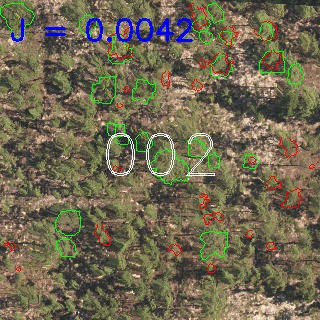
\includegraphics[height=1.8in]{figure/top5_0.jpg} & 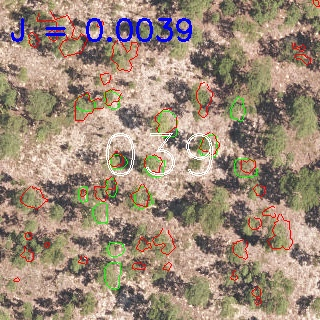
\includegraphics[height=1.8in]{figure/top5_1.jpg} & 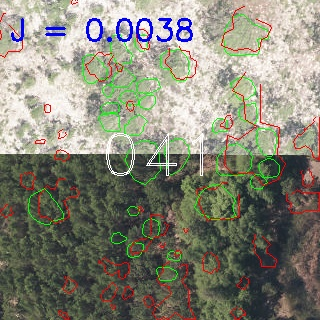
\includegraphics[height=1.8in]{figure/top5_2.jpg} \\
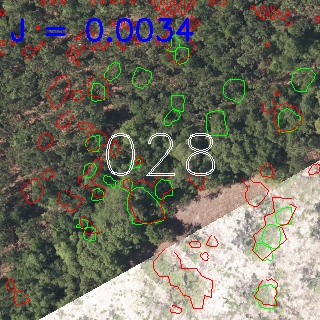
\includegraphics[height=1.8in]{figure/top5_3.jpg} & 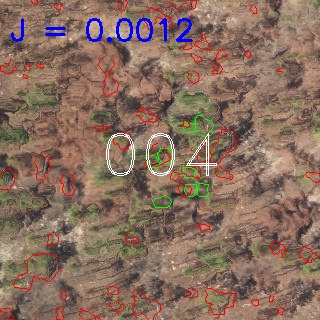
\includegraphics[height=1.8in]{figure/top5_4.jpg} & 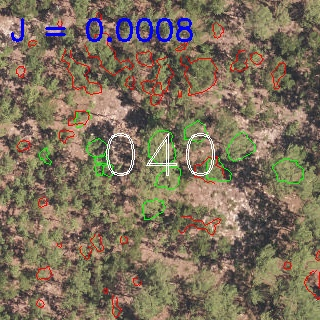
\includegraphics[height=1.8in]{figure/top5_5.jpg} \\
\end{tabular}
\end{table*}

\begin{table*}
\label{tab:top3}
\caption{The worst-6 Delineations}
\center
\begin{tabular}{lll}
\\
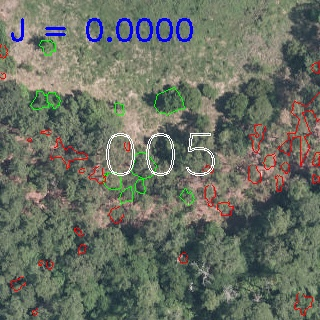
\includegraphics[height=1.8in]{figure/bottom5_0.jpg} & 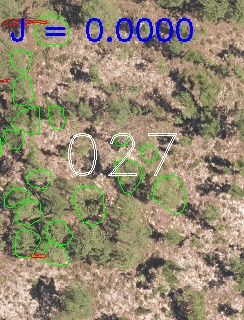
\includegraphics[height=1.8in]{figure/bottom5_1.jpg} & 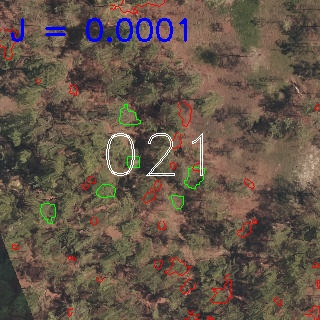
\includegraphics[height=1.8in]{figure/bottom5_2.jpg} \\
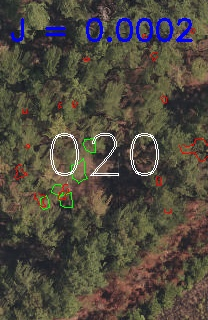
\includegraphics[height=1.8in]{figure/bottom5_3.jpg} & 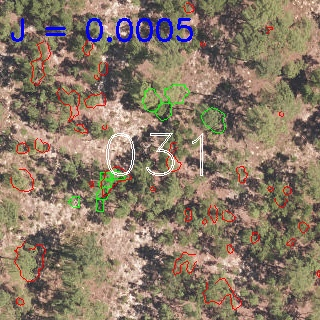
\includegraphics[height=1.8in]{figure/bottom5_4.jpg} & 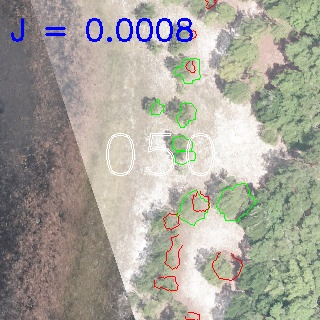
\includegraphics[height=1.8in]{figure/bottom5_5.jpg} \\
\end{tabular}
\end{table*}



\end{document}
